\documentclass[11pt,a4paper]{article}
\usepackage[utf8]{inputenc}\usepackage[T1]{fontenc}
\usepackage{amsmath, amssymb, amsthm}
\usepackage[margin=1in]{geometry}
\usepackage{hyperref}\usepackage{mathrsfs}\usepackage{graphicx}\usepackage{xcolor}
\hypersetup{hidelinks}
\newtheorem{proposition}{Proposition}
\newtheorem{lemma}{Lemma}
\newtheorem{definition}{Definition}

\title{\Large \textbf{The $6N$-Skeleton Zeta Function\\
and its Log-Periodic Zero-Ladders}}
\author{Ruqing Chen\\
\small GUT Geoservice Inc., Montreal, Quebec, Canada\\
\small \texttt{ruqing@hotmail.com}}
\date{\today}

\begin{document}
\maketitle

\begin{abstract}
The $6N$ skeleton is built by stripping the primes $2$ and $3$, so that every
remaining prime sits on a fault line $6N\pm1$. We make that stripping explicit at
the level of the zeta function. Removing the $q=2$ and $q=3$ Euler factors defines
$\zeta_{6N}(s)=\zeta(s)(1-2^{-s})(1-3^{-s})=\prod_{p\ge5}(1-p^{-s})^{-1}
=\sum_{\gcd(n,6)=1}n^{-s}$, the Dirichlet series of the integers coprime to $6$. Its
analytic structure is elementary but clean: a simple pole at $s=1$ with residue
$1/3$, and a zero set that splits into two orthogonal families---the non-trivial
zeros of $\zeta$ on the critical line $\beta=\tfrac12$, unchanged, and two
\emph{new} ladders of zeros on the imaginary axis $\beta=0$, at $s=2\pi i k/\ln 2$
and $s=2\pi i n/\ln 3$. Because $\ln2/\ln3$ is irrational the two ladders are
incommensurate, meeting only at the double zero $s=0$. We show these ladders are
exactly the Fourier modes of the two log-periodic staircases $\psi_2,\psi_3$ that
count the powers of $2$ and $3$ removed from $\psi(x)$; equivalently, the
skeleton's prime count $\psi_{6N}(x)=\sum_{p\ge5,\,p^k\le x}\ln p$ decomposes into a
smooth term, the fluctuating critical-line ($\beta=\tfrac12$) part, and a rigid,
exactly log-periodic ($\beta=0$) grid. We are explicit about scope: $\zeta_{6N}$ is
$\zeta$ with two Euler factors removed, its extra zeros are a construction artifact
of that removal, and nothing here bears on the Riemann Hypothesis or on the
infinitude of any prime constellation.
\end{abstract}

\section{Introduction}
Throughout this series the $6N$ skeleton has been defined operationally: discard the
primes $2$ and $3$, and every surviving prime ($>3$) lies at $6N\pm1$. Volumes I--II
worked with this skeleton combinatorially and in congruence phase space. Here we ask
the obvious complex-analytic question: what is the Dirichlet generating function of
the skeleton, and what does ``removing $2$ and $3$'' do to the zeros of $\zeta$?

The answer is modest and exact. Removing the two Euler factors multiplies $\zeta$ by
$(1-2^{-s})(1-3^{-s})$, which introduces two arithmetic-progression ladders of
zeros on the imaginary axis. These are not deep new zeros---they are the spectral
fingerprint of the two log-periodic staircases (the powers of $2$ and of $3$) that
the skeleton throws away. What is mildly satisfying is the clean separation that
results: a rigid periodic grid at $\beta=0$ and the familiar fluctuating zeros at
$\beta=\tfrac12$, sitting side by side in one generating function.

\section{Motivation: where the skeleton's prime energy lives}
Before defining $\zeta_{6N}$ we record the elementary fact that motivates removing
$2$ and $3$. The von Mangoldt weight $\Lambda(n)=\ln p$ for $n=p^k$ is supported on
prime powers; for $p\ge5$ these sit at $n\equiv\pm1\pmod6$, while the powers of $2$
and $3$ occupy the residues $\{2,4\}$ and $\{3\}$, and no prime power is $\equiv0$.
Binning $\sum_{n\le X}\Lambda(n)$ by residue mod $6$ at $X=10^7$
(Fig.~\ref{fig:energy}) shows $99.9997\%$ of the total weight on the fault lines
$6N\pm1$, split essentially evenly, with only $O(\log X)$ left on the powers of
$2,3$ and exactly nothing on the multiples of $6$.

\begin{figure}[h]\centering
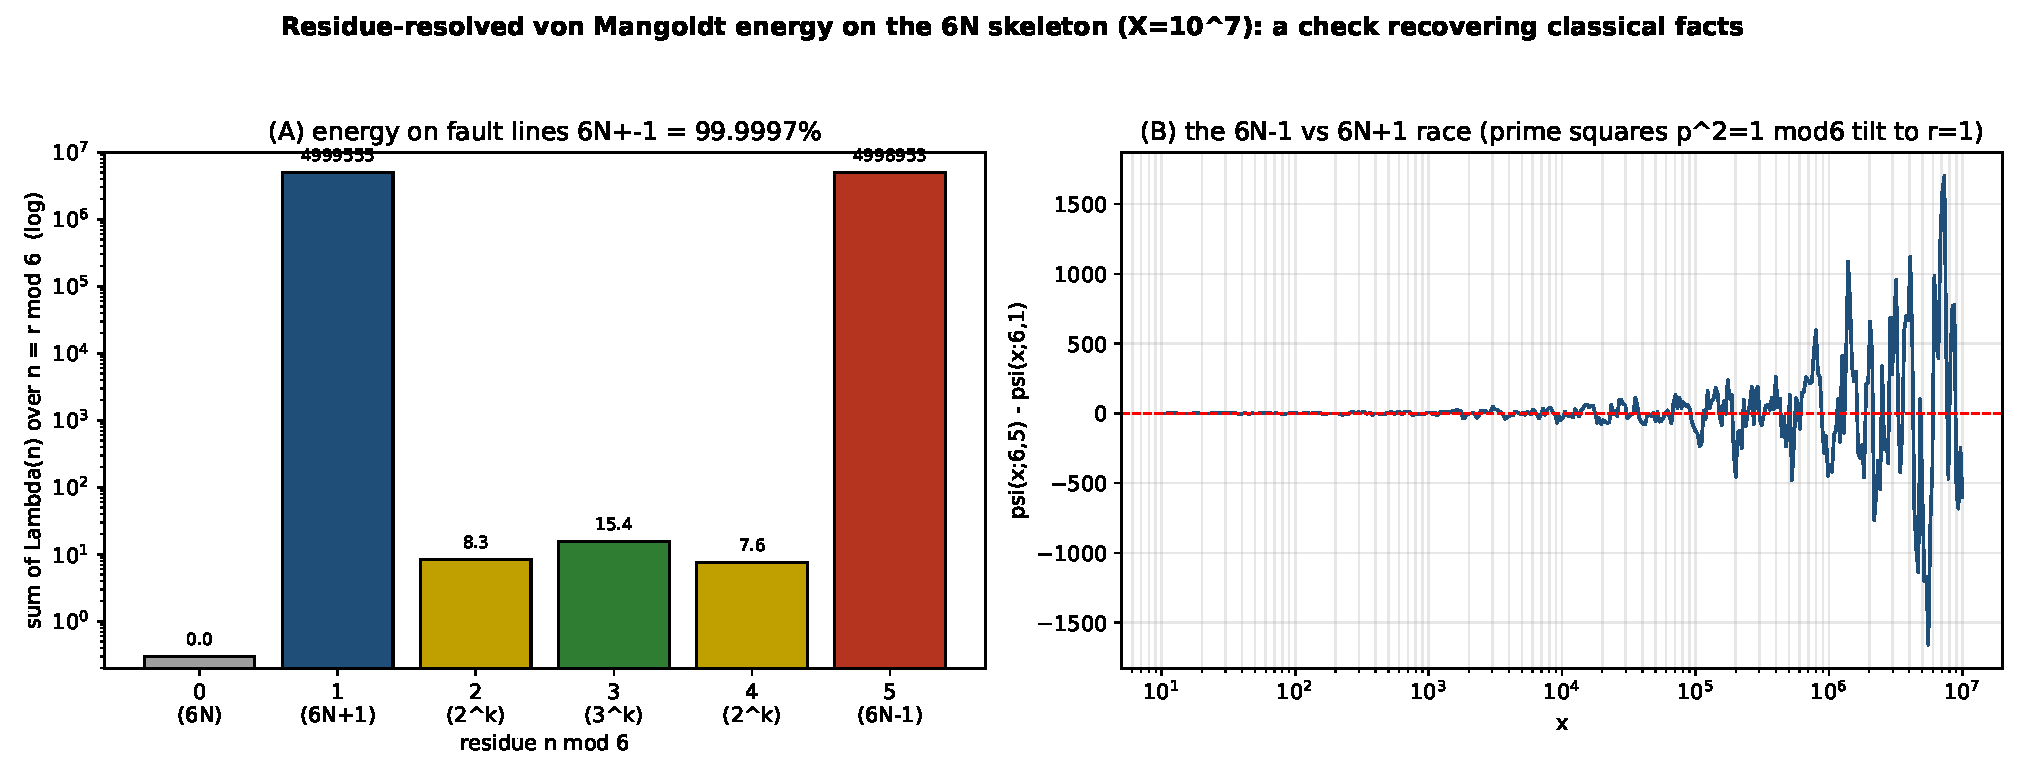
\includegraphics[width=0.96\textwidth]{fig_residue_energy.pdf}
\caption{(A) The von Mangoldt energy $\sum_{n\le X,\,n\equiv r}\Lambda(n)$ by residue
$r\bmod6$ at $X=10^7$: the fault lines $6N\pm1$ carry $99.9997\%$, the residues
$2,3,4$ only $O(\log X)$ (powers of $2,3$), and $r=0$ nothing. (B) The
$6N{-}1$ vs $6N{+}1$ race $\psi(x;6,5)-\psi(x;6,1)$, oscillating at scale
$O(\sqrt x)$. These are the classical facts---prime distribution in arithmetic
progressions and its $\sqrt x$ fluctuation---displayed on the skeleton; they are
not new, and we use them only to justify isolating the $6N\pm1$ generators.}
\label{fig:energy}
\end{figure}

This is exactly the prime number theorem in the arithmetic progressions
$\pmod 6$~\cite{Davenport}, with the $\sqrt x$-scale race a face of the explicit
formula. We claim no novelty here; it is the empirical reason to define a generating
function that keeps only the $p\ge5$ factors.

\section{The $6N$-skeleton zeta function}
\begin{definition}
For $\mathrm{Re}(s)>1$,
\begin{equation}
  \zeta_{6N}(s)\;:=\;\zeta(s)\,(1-2^{-s})(1-3^{-s})
  \;=\;\prod_{p\ge5}\bigl(1-p^{-s}\bigr)^{-1}
  \;=\!\!\sum_{\substack{n\ge1\\ \gcd(n,6)=1}}\!\! n^{-s},
\end{equation}
the Dirichlet series of the integers coprime to $6$ (equivalently, the
$5$-rough integers). It continues meromorphically to $\mathbb{C}$ through $\zeta$.
\end{definition}

\begin{proposition}[Pole]
$\zeta_{6N}$ has a single simple pole, at $s=1$, with residue
$(1-\tfrac12)(1-\tfrac13)=\tfrac13$, reflecting the density $\varphi(6)/6=1/3$ of the
integers coprime to $6$.
\end{proposition}
\begin{proof}
$\zeta$ has a simple pole at $s=1$ with residue $1$; the analytic factor
$(1-2^{-s})(1-3^{-s})$ takes the value $\tfrac12\cdot\tfrac23=\tfrac13$ there and is
holomorphic, so the residue is $1\cdot\tfrac13$.
\end{proof}

\section{The zero set: a critical-line family and two imaginary ladders}
Since $\zeta_{6N}=\zeta\cdot(1-2^{-s})(1-3^{-s})$, its zeros are the union of the
zeros of the three factors.

\begin{proposition}[Zero set]\label{prop:zeros}
The zeros of $\zeta_{6N}$ are:
\begin{enumerate}
\item the non-trivial zeros $\rho=\tfrac12+i\gamma$ of $\zeta$ (unchanged), together
  with the trivial zeros $s=-2,-4,\dots$;
\item the ladder $L_2=\{\,2\pi i k/\ln2 : k\in\mathbb{Z}\,\}$, from $1-2^{-s}=0$;
\item the ladder $L_3=\{\,2\pi i n/\ln3 : n\in\mathbb{Z}\,\}$, from $1-3^{-s}=0$.
\end{enumerate}
Both ladders lie on the imaginary axis $\beta=0$, with constant spacings
$2\pi/\ln2\approx9.0647$ and $2\pi/\ln3\approx5.7192$. Since $\ln2/\ln3$ is
irrational, $L_2\cap L_3=\{0\}$, where the two simple zeros coincide into a double
zero of $\zeta_{6N}$.
\end{proposition}

\begin{figure}[h]\centering
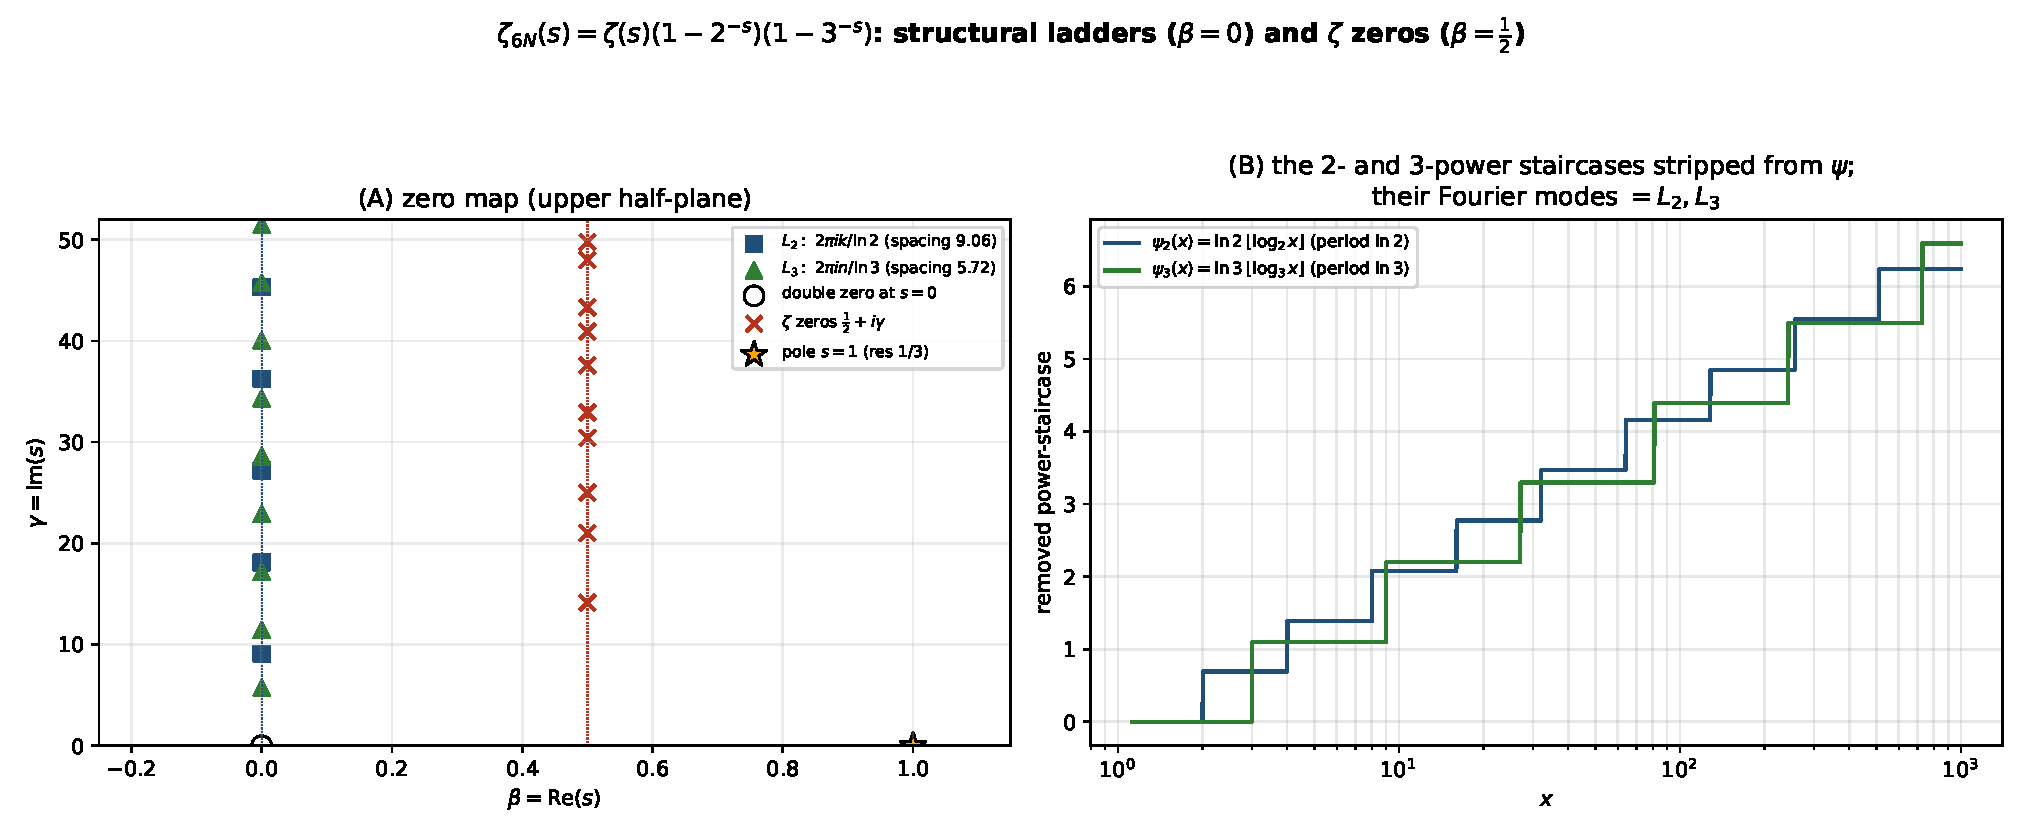
\includegraphics[width=0.96\textwidth]{fig_zeta6n.pdf}
\caption{(A) Zero map of $\zeta_{6N}$ (upper half-plane): the incommensurate
imaginary ladders $L_2$ (spacing $9.06$) and $L_3$ (spacing $5.72$) at $\beta=0$,
the double zero at $s=0$, the critical-line zeros $\tfrac12+i\gamma$ of $\zeta$, and
the pole at $s=1$. (B) The log-periodic staircases $\psi_2(x)=\ln2\lfloor\log_2
x\rfloor$ and $\psi_3(x)=\ln3\lfloor\log_3 x\rfloor$ removed from $\psi$; their
Fourier frequencies are precisely $L_2$ and $L_3$.}
\label{fig:zeros}
\end{figure}

\section{The ladders are the Fourier modes of the removed staircases}
The two new families are not arithmetic accidents; they are the spectrum of what the
skeleton discards. The skeleton's prime count is
\begin{equation}
  \psi_{6N}(x)=\!\!\sum_{\substack{p\ge5\\ p^k\le x}}\!\!\ln p
  \;=\;\psi(x)-\psi_2(x)-\psi_3(x),\qquad
  \psi_2(x)=\ln2\Big\lfloor\tfrac{\ln x}{\ln2}\Big\rfloor,\;\;
  \psi_3(x)=\ln3\Big\lfloor\tfrac{\ln x}{\ln3}\Big\rfloor,
\end{equation}
where $\psi_2,\psi_3$ are staircases of period $\ln2,\ln3$ in $\ln x$. Their
contribution to the logarithmic derivative is
\begin{equation}
  -\frac{d}{ds}\ln(1-2^{-s})
  =-\ln2\sum_{k\ge1}(2^{k})^{-s},
\end{equation}
the Dirichlet series supported on powers of $2$; the zeros $L_2$ of $1-2^{-s}$ are
exactly the frequencies of the Fourier expansion of the sawtooth $\{\log_2 x\}$, and
likewise $L_3$ for $3$. Reading $\psi_{6N}$ through the explicit formula therefore
gives a clean three-way split:
\begin{equation}
  \psi_{6N}(x)\;=\;\underbrace{x}_{\text{smooth}}
  \;-\;\underbrace{\sum_{\rho}\frac{x^{\rho}}{\rho}}_{\beta=\frac12\ \text{fluctuation}}
  \;-\;\underbrace{\big(\psi_2(x)+\psi_3(x)\big)}_{\beta=0\ \text{log-periodic grid}}
  \;+\;\text{(lower order)}.
\end{equation}
The $\beta=0$ ladders form a rigid, exactly periodic grid (the discarded $2,3$
residues); the $\beta=\tfrac12$ zeros carry the fluctuation. In this precise sense
the structural and the fluctuating parts of the skeleton's prime count are
orthogonal: one is a finite-rate set of pure log-frequencies, the other the
critical-line spectrum.

\section{Conclusion}
The $6N$-skeleton zeta function $\zeta_{6N}(s)=\zeta(s)(1-2^{-s})(1-3^{-s})$ is the
generating function of the integers coprime to $6$. Its only departures from $\zeta$
are bookkeeping consequences of removing the $2$ and $3$ Euler factors: the residue
at $s=1$ shrinks to $1/3$, and two incommensurate ladders of zeros appear on the
imaginary axis, encoding the log-periodic staircases of powers of $2$ and $3$. The
resulting separation---a rigid $\beta=0$ grid beside the fluctuating $\beta=\tfrac12$
zeros---is a tidy way to see what the skeleton keeps and what it throws away. We
stress the limits of the claim: this is an elementary modification of $\zeta$, the
new zeros are construction artifacts rather than discoveries, and the framework says
nothing about the Riemann Hypothesis or the infinitude of primes or prime
constellations beyond what classical theory already gives.

\paragraph{Data and code availability.}
The residue-energy computation, the zero-map and staircase figure, and a verifier of
$\zeta_{6N}$'s pole, ladders, and incommensurability are openly available at
\url{https://github.com/Ruqing1963/6N-skeleton-zeta}~\cite{repo}.

\begin{thebibliography}{9}
\bibitem{Riemann} B.~Riemann, \emph{Ueber die Anzahl der Primzahlen unter einer
gegebenen Gr\"osse}, Monatsber.\ Berlin Akad.\ (1859).
\bibitem{Davenport} H.~Davenport, \emph{Multiplicative Number Theory}, 3rd ed.,
Springer GTM~74 (2000).
\bibitem{ChenV} R.~Chen, Part~V, Zenodo, doi:10.5281/zenodo.20510700 (2026).
\bibitem{ChenXX} R.~Chen, \emph{The circular convolution of prime constellations in
congruence phase space} (Part~XX), Zenodo, doi:10.5281/zenodo.20583994 (2026).
\bibitem{ChenXXIV} R.~Chen, \emph{The quasi-periodic diffraction spectrum of
twin-pair correlation on the $6N$ skeleton} (Part~XXIV), Zenodo,
doi:10.5281/zenodo.20587185 (2026).
\bibitem{Review} R.~Chen, \emph{Arithmetic geodynamics on the $6N$ skeleton: a
review of Parts I--XIX}, Zenodo, doi:10.5281/zenodo.20585301 (2026).
\bibitem{repo} R.~Chen, \emph{The $6N$-skeleton zeta function and its log-periodic
zero-ladders} (Part~XXV),
\url{https://github.com/Ruqing1963/6N-skeleton-zeta} (2026).
\end{thebibliography}

\end{document}
